\section{Basic Assumptions}
Suppose a particle can be described by a probability distribution over space $x$ and time $t$, then the ``uniform'' particle is described by a plane wave
\begin{align}
\psi \propto \exp\left(
i~\dfrac{px-Et}{\hbar}
\right),
\end{align}
with constant momentum $p$ and energy $E$. The imaginary $i$ is needed to keep the amplitude of this wave $\psi^*\psi$ constant, whereas $\hbar$ is needed to remove units from the exponent. From derivatives of this plane wave, it is natural to conjecture the relations of conjugate variables to space and time, i.e. momentum and energy
\begin{align}
\left\{
\begin{array}{l}
\frac{d\psi}{dx} =  i\frac{p}{\hbar}\psi \\ [8 pt]
\frac{d\psi}{dt} = -i\frac{E}{\hbar}\psi
\end{array}
\right. \Rightarrow
\left\{
\begin{array}{l}
p\psi = -i\hbar\frac{d}{dx} \psi \\ [8 pt]
E\psi =  i\hbar\frac{d}{dt} \psi
\end{array}
\right..
\end{align}
Suppose total energy is a sum of non-relativist kinetic energy and local potential energy
\begin{align}
E = \frac{p^2}{2m} + V(x),
\end{align}
then the Hamiltonian operator
\begin{align}
\hat{\mathcal{H}} = \frac{\hat{p^2}}{2m} + V(x) = -\frac{\hbar^2}{2m}\nabla^2 + V(x).
\end{align}

\section{Introduction}
%Exact simulation of electron-ion systems is the grand challenge of this century.
Exact simulation of the homogeneous electron gas was the holy grail of the last century. It has led to quantitative understanding of metals and semiconductors as well as the popular local density approximation of the density functional which opened the flood gates on countless materials simulations. However, the grand challenge of this century is the exact simulation of electron-ion systems.
While the jellium model mimic many essential features of electrons in real materials, valence electrons in real materials interact with point charges (nuclei) and the surrounding inner electrons that screen them.
To complicate matters, these nuclei form a crystalline arrangement only on average. They move around and can change the electronic structure significantly. Even at absolute zero, the zero-point motion of the ions can still be the deciding factor of the stability between two candidate crystal structures.
The electron-ion problem is far from being solved.
Along with excited states.

The quantum liquids helium and jellium are at the forefront of the quantum era ushered in the last century.
Having stable closed-shells, helium atoms interact mostly via an isotropic pair potential. It consists of a $r^{-6}$ van der Waals attraction at long range due to correlated dipole fluctuation and a hard-core repulsion upon electron density overlap~\cite{Aziz1979}.
Thus, the electronic problem is removed and only the ionic problem remains
\begin{align}
\hat{H}_{He} = \sum\limits_{I=1}^{N_I} -\dfrac{\hbar^2}{2m_I}\nabla_I^2
+\frac{1}{2}\sum\limits_{I=1}^{N_I}\sum\limits_{J=1,J\neq I}^{N_I} v(\vert\ri-\rj\vert).
\end{align}
In the opposite extreme, 
\begin{align}
\dfrac{1}{n} \equiv \dfrac{\Omega}{N} = \left\{\begin{array}{lr}
2 r_s a_B & 1D\\
\pi(r_sa_B)^2 & 2D\\
\frac{4\pi}{3}(r_sa_B)^3 & 3D
\end{array}\right.,
\end{align}

%\subsection{Exact Electron-Ion Schr\"odinger equations towards Born-Oppenheimer}


\begin{comment}
\begin{table}[h]
\centering
\begin{tabular}{cccccc}
\toprule
     & Temperature & Classical & Quantum & Quantization & Sign Problem \\
\midrule
PIMC &     any     &   yes     &   yes   & first & $\braket{\sigma}\propto \exp\left[ -\beta N (F_f-F_b) \right]$ \\
DMC  &    zero     &    no     &   yes   & first & $\braket{\sigma}\propto \exp\left[ -\beta N (F_f-F_T) \right]$ \\
FP-DMC & zero & no & yes & first & no \\
VMC & low & no & yes & first & no \\
AFQMC & low & no & yes & second & ? \\
\bottomrule
\end{tabular}
\end{table}
\end{comment}

The electron-ion pair correlation functions are shown in Fig.~\ref{fig:hsolid-epgr}.
They are shown separately for each candidate structure with pressure encoded in color.
For all candidate structures, the small-distance electron-proton correlation decrease as pressure increases.
As the kinetic energy becomes more important, the electrons delocalize more to lower kinetic energy, thus localize less around the protons.

\begin{figure}[h]
\centering
\begin{minipage}{0.49\textwidth}
\centering
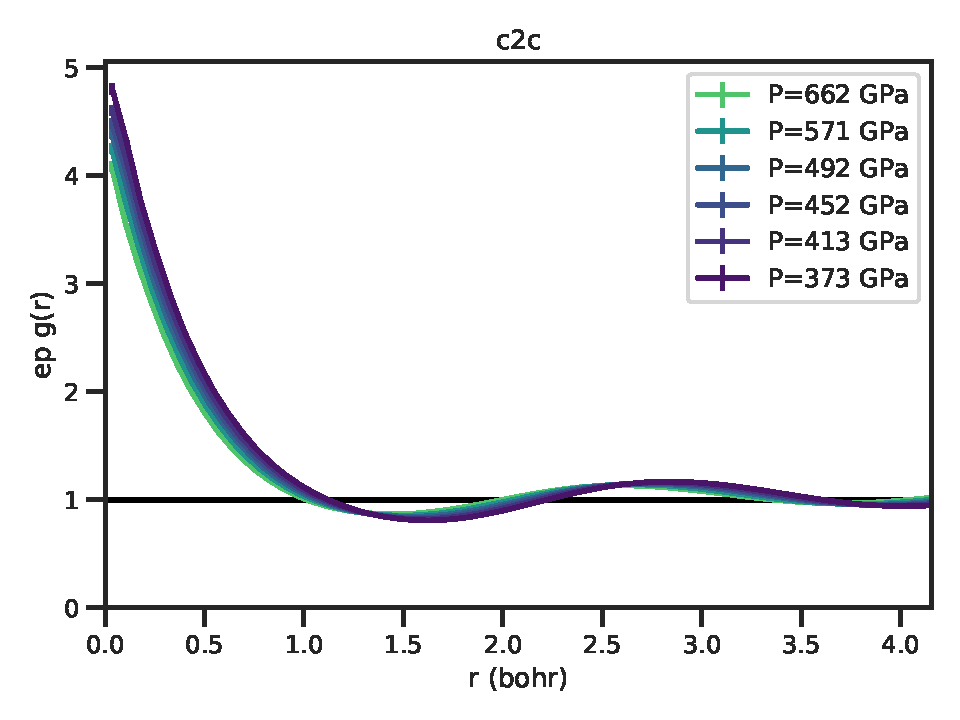
\includegraphics[width=\linewidth]{h117ga_dynamic-c2c-s2-ep}\\
(a) C2/c-24
\end{minipage}
\begin{minipage}{0.49\textwidth}
\centering
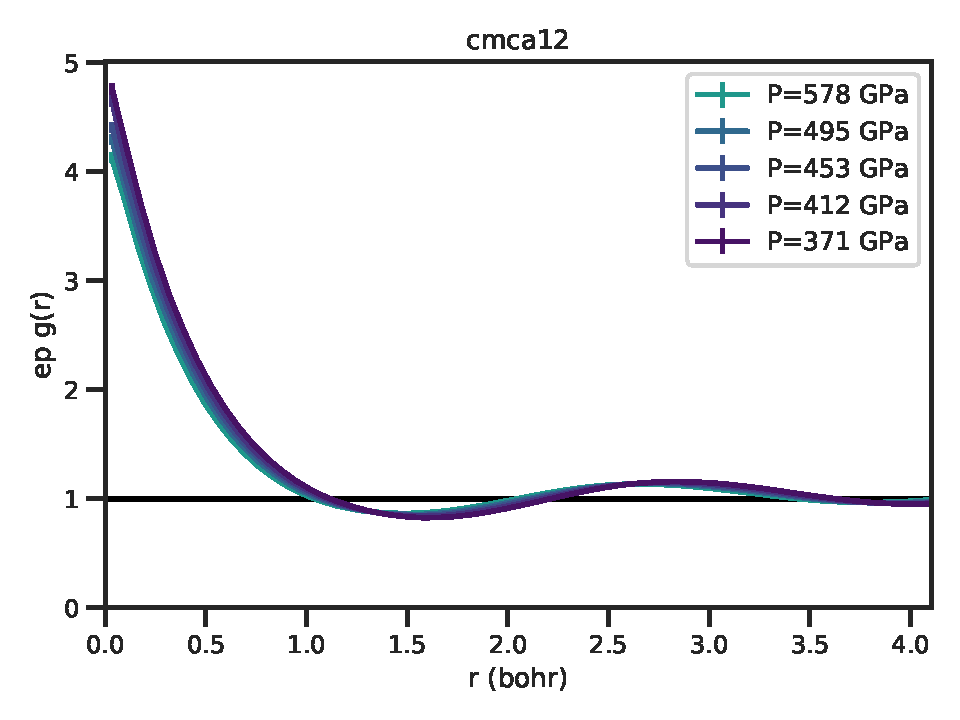
\includegraphics[width=\linewidth]{h117ga_dynamic-cmca12-s2-ep}\\
(b) Cmca-12
\end{minipage}
\begin{minipage}{0.49\textwidth}
\centering
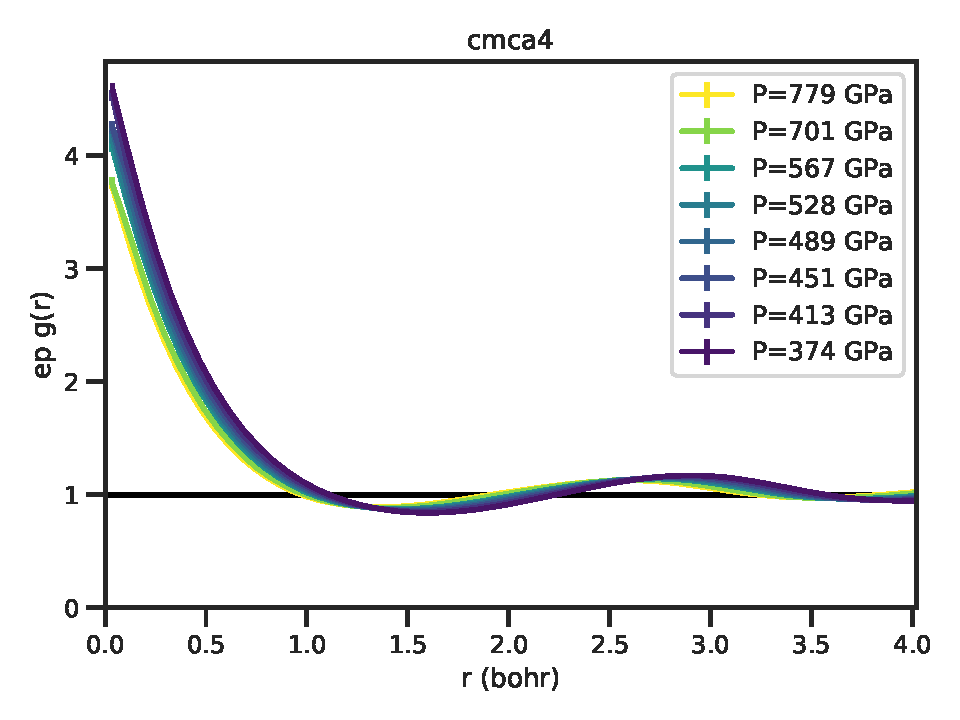
\includegraphics[width=\linewidth]{h117ga_dynamic-cmca4-s2-ep}\\
(c) Cmca-4
\end{minipage}
\begin{minipage}{0.49\textwidth}
\centering
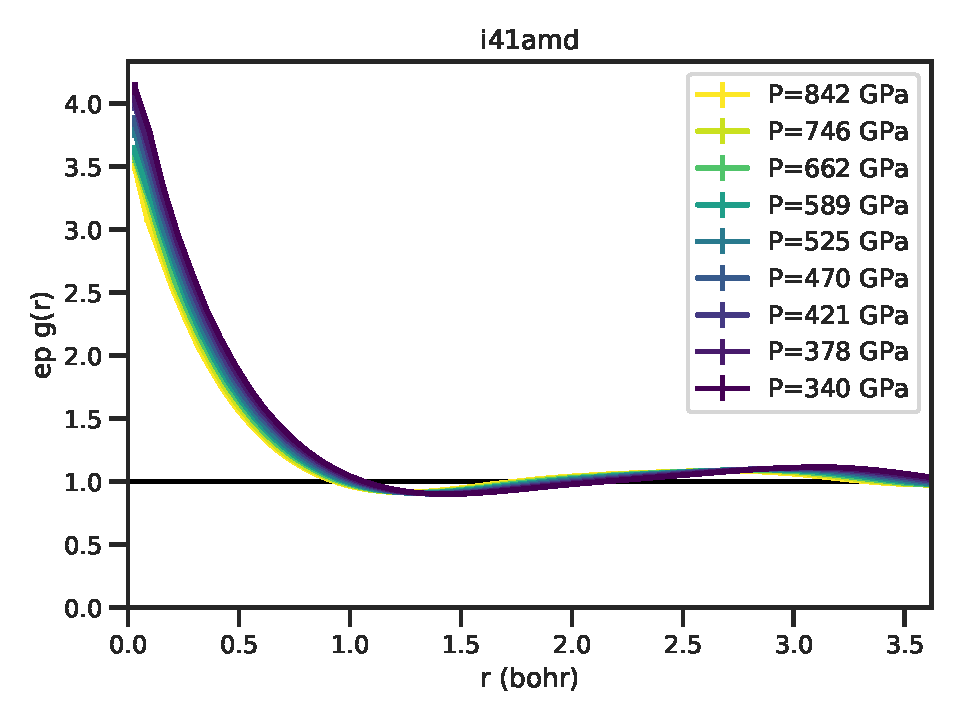
\includegraphics[width=\linewidth]{h117ga_dynamic-i41amd-s2-ep}\\
(d) I4$_1$/amd
\end{minipage}
\caption{Dynamic-lattice electron-proton pair correlation function ep $g(r)$.}
\label{fig:hsolid-epgr}
\end{figure}

%The goal is to combine and improve upon the best methods in all previous QMC studies and provide the most accurate properties of the solid hydrogen phases.

%\subsection{The melting transition and critical point}
%
%The melting temperature of solid hydrogen is typically determined in one of three ways: 1. visual observation of motion due to sample, contaminant, or laser speckle~\cite{Gregoryanz2003}, 2. discontinuous change in the Raman spectrum, e.g. vibron frequency jump, disappearance of librons~\cite{Gregoryanz2003,Subramanian2011,Zha2017}, 3. plateau temperature during laser heating~\cite{Deemyad2008}, and 4. rapid change in interferences pattern~\cite{Eremets2009}.
%As sample size decreases with pressure, visual detection of melting becomes more difficult. Further, the refractive indexes of hydrogen and diamond approach each other around 140 GPa, defeating detection by interference pattern~\cite{Zha2017}.
%The vibron discontinuity caused by melting reduces from $\sim$ 3 cm$^{-1}$ at 10 GPa to $\sim$ 1 cm$^{-1}$ at 45 GPa~\cite{Gregoryanz2003}, making melting detection more difficult at higher pressures.
%Finally, disappearance of librons alone cannot be taken as proof of melting, because it could be due to loss of sample.
%Due to these difficulties, the precise melting temperatures above 100 GPa are debate. Although, there is broad consensus that the melting line increases from 200 K at ambient pressure to $\sim$ 1000 K at 90 GPa, then decreases with increasing pressure.
%
%Melting of $H_2$ solid around 150 GPa is particularly interesting. Shock wave compression data indicate a molecular liquid to atomic liquid transition $\sim$ 1000 K at 150 GPa. Thus, $H_2$ molecules should dissociate almost immediately after the solid melts. Eremets and Trojan observed a shark drop in measured resistivity as the $H_2$ solid melts at 146 GPa~\cite{Eremets2009}. This observation is consistent with the current liquid-liquid transition (LLT) line.